%-------------------------------------------------------------------------------
%							PREAMBULE
%-------------------------------------------------------------------------------

\documentclass[9pt,xcolor=dvipsnames]{beamer} % dvipsnames gives more built-in colors

\usetheme{Szeged}
\useoutertheme{miniframes} % Alternatively: miniframes, infolines, split, smoothbars, smoothtree, shadow
\useinnertheme{rectangles}

\usepackage{media9}
\usepackage{graphicx}

\usepackage{docmute} % To include multiple files

\usepackage{tikz}
\usetikzlibrary{positioning,shapes,arrows}
\usetikzlibrary{babel}      % Utiliser ce Babel pour eviter les problemes avec les animations TIKX
% \usepackage{csquotes}

\graphicspath{ {./Figures/} }
\usepackage[utf8]{inputenc}
\usepackage{amsmath,bm,mathtools}
% \usepackage{unicode-math}
\usepackage{cases}
\usepackage{siunitx}

\usepackage[T1]{fontenc}
\usepackage{iwona}    %% Roman text font 
\usepackage{mathdots}
\usepackage{eulervm}    %% De eres droits symboles mathmatiques

\newcommand{\bvec}[1]{\bm{#1}}    %% For vector notation
\newcommand{\myvec}[2]{\begin{pmatrix} #1  \\ #2 \end{pmatrix}}   %% vecteur 2d
\newcommand{\mymat}[4]{\begin{pmatrix} #1 & #2 \\ #3 & #4 \end{pmatrix}}  %% Matrice 2*2

\usepackage[backend=bibtex,style=authoryear,maxnames=2,natbib=true]{biblatex} % Use the bibtex backend with the authoryear citation style (which resembles APA)
\addbibresource{bibliography.bib} % The filename of the bibliography
\usepackage[autostyle=true]{csquotes} % Required to generate language-dependent quotes in the bibliography 
\renewcommand*{\bibfont}{\tiny} % Pour reduire la taille des references

\usepackage[font=scriptsize]{caption}
% \captionsetup{labelformat=empty,labelsep=none}    % Pour retirer le terme figure des titres

\usepackage{hyperref}
\usepackage{booktabs}

\usepackage{etoolbox}
\newcommand{\zerodisplayskips}{%        %% To remove space after math box
  \setlength{\abovedisplayskip}{0pt}%
  \setlength{\belowdisplayskip}{0pt}%
  \setlength{\abovedisplayshortskip}{0pt}%
  \setlength{\belowdisplayshortskip}{0pt}}
% \appto{\normalsize}{\zerodisplayskips}
% \appto{\small}{\zerodisplayskips}
% \appto{\footnotesize}{\zerodisplayskips}
\newcommand{\phifem}{$\phi$-FEM }

\beamertemplatenavigationsymbolsempty   %% Remove nav symbols

%-------------------------------------------------------------------------------
%							IMPORTANT TRANPARENCY AND COLOR DEFINTION 
%-------------------------------------------------------------------------------
\definecolor{MyGreen}{RGB}{0, 50, 0}
\definecolor{MyRed}{rgb}{0.85, 0, 0}
\definecolor{MyPurple}{rgb}{0.7, 0.1, 0.7}
\definecolor{MyGrey}{rgb}{0.7, 0.75, 0.71}
\definecolor{MyTitleGreen}{rgb}{0.67, 0.88, 0.69}

\usecolortheme[named=MyGreen]{structure} % Base color for the slides
\setbeamercolor{alerted text}{fg=MyRed}
\setbeamercolor{section in head/foot}{bg=MyGrey}
\setbeamercolor{titlelike}{parent=structure,bg=MyGrey}  %% For frametiles

\setbeamercolor{date in head/foot}{bg=MyGrey}
\setbeamercolor{author in head/foot}{bg=MyGrey}
\setbeamercolor{subsection in head/foot}{bg=MyTitleGreen}

\setbeamercovered{transparent}    %% Pour avoir de la tranparence

\setbeamertemplate{subsection in head/foot}{}

% ## Set color for blocks and examples
\setbeamercolor{block title}{use=structure,fg=white,bg=structure.fg!75!black}
\setbeamercolor{block title alerted}{use=alerted text,fg=white,bg=alerted text.fg!75!black}
\setbeamercolor{block title example}{use=example text,fg=white,bg=example text.fg!75!black}

\setbeamercolor{block body}{parent=normal text,use=block title,bg=block title.bg!10!bg}
\setbeamercolor{block body alerted}{parent=normal text,use=block title alerted,bg=block title alerted.bg!10!bg}
\setbeamercolor{block body example}{parent=normal text,use=block title example,bg=block title example.bg!10!bg}


%-------------------------------------------------------------------------------
%							A CUSTOM FOOTLINE
%-------------------------------------------------------------------------------

\makeatletter
\setbeamertemplate{footline}{
	\begin{beamercolorbox}[colsep=1.5pt]{upper separation line foot}
	\end{beamercolorbox}
  \leavevmode%
  \hbox{%
  \begin{beamercolorbox}[wd=.333333\paperwidth,ht=2.25ex,dp=1ex,center]{author in head/foot}%
	% \usebeamerfont{author in head/foot}\insertshortauthor\expandafter\beamer@ifempty\expandafter{\beamer@shortinstitute}{}{~~(\insertshortinstitute)}
	\insertshortauthor
  \end{beamercolorbox}%
  \begin{beamercolorbox}[wd=.333333\paperwidth,ht=2.25ex,dp=1ex,center]{title in head/foot}%
    \usebeamerfont{title in head/foot}\insertshorttitle
  \end{beamercolorbox}%
  \begin{beamercolorbox}[wd=.333333\paperwidth,ht=2.25ex,dp=1ex,right]{date in head/foot}%
    \usebeamerfont{date in head/foot}\insertshortdate{}\hspace*{2em}
    \insertframenumber{} / \inserttotalframenumber\hspace*{2ex} 
  \end{beamercolorbox}}%
  \vskip0pt%

  \begin{beamercolorbox}[colsep=1.5pt]{lower separation line foot}
  \end{beamercolorbox}

}
\makeatother


%-------------------------------------------------------------------------------
%							TITLE PAGE
%-------------------------------------------------------------------------------
\begin{document}


\title[Transfert radiatif]{Reconstruction de la densité d'un domaine par un Vnet }

% \institute[Université de Strasbourg]{\small \textbf{ \hspace*{0.1mm} Referent teacher} \hspace*{11mm} \textbf{Supervisors} \\ \footnotesize Christophe PRUD'HOMME \hspace*{4mm} Michel DUPREZ \\ \hspace*{38mm} Stephane COTIN}
\institute[Université de Strasbourg]{\normalsize \textbf{Superviseurs} \\ Vincent VIGON - Emmanuel FRANCK - Laurent NAVORET}

% \institute[University of Strasbourg]{\normalsize \textbf{Enseignant} \\ Pr. Yannick PRIVAT}

\author[Desmond Roussel NGUEGUIN]{\textbf{Étudiant} \\ Desmond Roussel NGUEGUIN}
% \date[\today]{\textbf{Unités d'enseignement} \\ Traitement de signal 2 - Projet \\ \vspace*{0.2cm} \textbf{Année universitaire 2020/2021}}
\date[\today]{\textbf{Année universitaire 2020/2021}}

\begingroup  % A new group whose informations are not cannon. Just for convenience
\setbeamertemplate{navigation symbols}{}
\setbeamertemplate{headline}{\vspace{0.5cm}%
  \hspace*{0.8cm}%
  
\includegraphics[width=2.8cm]{LogoUnistra}
  \hfill\raisebox{.2cm}{\normalsize  }\hfill%
  
\includegraphics[width=2.1cm]{LogoIRMA.png}
  \hfill\raisebox{.2cm}{\normalsize  }\hfill%
  
\includegraphics[width=2.5cm]{LogoCSMI}
  \hspace*{0.8cm}%
}
\begin{frame}[fragile]
\maketitle
\end{frame}
\endgroup



%-------------------------------------------------------------------------------
%							SECTION TITLE slides
%-------------------------------------------------------------------------------


\AtBeginSection[]{
  \begin{frame}
  \vfill
  \centering
  \begin{beamercolorbox}[sep=8pt,center,shadow=true,rounded=true]{title}
    \usebeamerfont{title}\insertsectionhead\par%
  \end{beamercolorbox}
  \vfill
  \end{frame}
}


%-------------------------------------------------------------------------------
%							INCLUDE THE CHAPTERS
%-------------------------------------------------------------------------------

\begin{frame}
  \small
  \frametitle{Sommaire}
  \tableofcontents
\end{frame}


%-------------------------------------------------------------------------------
%							FIRST SECTION
%-------------------------------------------------------------------------------

\section{Le projet MOCO}


\begin{frame}
    \frametitle{Un résumé du stage}

Ce projet s'inscrit dans la suite du stage de M1 "\textbf{Simulation 2D de l’équation du transfert radiatif et reconstruction de la densité par un réseau de neurones}". 

\pause
\vspace{0.5cm}
Quelques améliorations faites:

    \begin{itemize}
        \item Code volume finis 1D simple $\rightarrow$ 2D simple $\rightarrow$ 2D avec entrées \textbf{Numpy} \pause
        \item CNN $\rightarrow$ Vnet  \pause
        \item On reconstruit la totalité de la densité du domaine, et non des créneaux
    \end{itemize}

\pause
\vspace{0.5cm}

\href{https://github.com/desmond-rn/projet-inverse-2d/blob/master/Rapport.pdf}{👉 \Large \alert{Lien vers le rapport de stage}.} 

\end{frame}


%-------- Vrai debut de l'introduction (PB INVERSE)
\begin{frame}
    \frametitle{Pour situer le stage (et ce projet)}
  
    \begin{enumerate}[<+>]
      \item Explosion du Deep Learning % Depuis le debut de la decenie 2010, le Machine Learning a considerablement pris de l’ampleur (2015 a l’ILSVRC, etc..)
      %%%%%% IMAGE DU DEEP LEARNING
      \item Application du Machine Learning en imagerie médicale % Avant de soigner les cancers, on doit detecter les tumeurs sont plus denses que les tissus sains (Chercher d'autres applications)
      %%%%%% IMAGE DU MEDICAL
      \item Réévaluation des méthodes de résolution des problèmes inverses % Les problemes inverses sont difficiles. ... Les algo d'optimisation classiques marchent tres bien. En fait on s'est referer aux travaux de Maya et Guillaume Dolle. L'avantage que peuvent offrir les ANN c'est juste la simplicite, et la rapidite, et une generalisation (non specificite aux probleme)
      %%%%%% IMAGE DU PB INVERSE
    \end{enumerate}
    
  \end{frame}

\begin{frame}
  \frametitle{Le(s) problème(s) à résoudre}

  \pause

\begin{columns}
 \begin{column}{0.5\textwidth}
  \centering
    Problème direct \\ (\scriptsize Résolution de l'ETR par un schéma de "splitting")
    % Image de densite -> signal sur les bords
      % 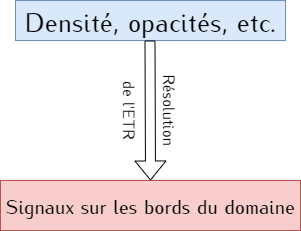
\includegraphics[width=5cm]{ProblemeDirect}       
  \end{column}

  \pause

 \begin{column}{0.5\textwidth}
    \centering
    Problème inverse \\ (\scriptsize Reconstruction de la densité par un réseau de neurones)
    %Image de signal sur les bords -> densite
      % 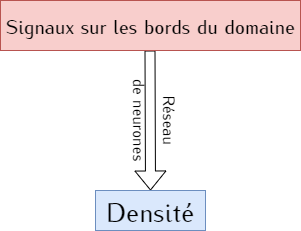
\includegraphics[width=5cm]{ProblemeInverse}       
 \end{column}
\end{columns}

\begin{figure}
  \includegraphics<1->[width=4cm]{PBInverse}         
\end{figure}

\end{frame}





\begin{frame}[fragile]
    \frametitle{Rappel des prédictions obtenues durant le stage (CNN)}

    \begin{columns}
    \begin{column}{0.5\textwidth}
        \begin{figure}
        \includegraphics<1->[width=3cm]{Meilleur2D1}       
        \includegraphics<1->[width=3cm]{Meilleur2D2}       
        \only<1-> {\caption{Les meilleures prédictions}}
        \end{figure}
     \end{column}
     \begin{column}{0.5\textwidth}
        \begin{figure}
        \includegraphics<2>[width=2.5cm]{Pire2D1}       
        \includegraphics<2>[width=2.5cm]{Pire2D2}       
        \includegraphics<2>[width=2.5cm]{Pire2D3}       
        \only<2>{\caption{Les pires prédictions}}
        \end{figure}
     \end{column}
    \end{columns}

\end{frame}

\begin{frame}
    \frametitle{Les scores obtenus par le CNN}

    \begin{table}[h!]
        \centering
        \begin{tabular}{l l}
        \toprule
        \textbf{Nom du score} & \textbf{Valeur} \\
        \midrule
        R2 & 98.81 \%\\
        Personnalisé & 93.50 \%\\
        \bottomrule\\
        \end{tabular}
    \end{table}

    \begin{columns}
        \begin{column}{0.333\textwidth}
            \begin{figure}
            \includegraphics<2->[width=2cm]{PositionX2D}       
            \only<2->{\caption{Corrélation des abscisses}}
            \end{figure}
         \end{column}
         \begin{column}{0.333\textwidth}
            \begin{figure}
            \includegraphics<3->[width=2cm]{PositionY2D}       
            \only<3->{\caption{Corrélation des ordonnées}}
            \end{figure}
         \end{column}
         \begin{column}{0.333\textwidth}
            \begin{figure}
            \includegraphics<4->[width=2cm]{Hauteur2D}       
            \only<4->{\caption{Corrélation des hauteurs}}
            \end{figure}
         \end{column}
    \end{columns}

\end{frame}


\begin{frame}
    \frametitle{Quelques mots sur la régression par le CNN}
Détection de toutes les variables :
\begin{itemize}[<+>]
    \item L'abscisse, l'ordonnée, et la hauteur sont relativement bien prédits
    \item La valeur de la densité en dehors du créneau est \textbf{fixée} :\\ $\Rightarrow$ \alert {\textbf{pas vraiment une reconstruction complète de la densité du milieu}}
\end{itemize}
\end{frame}

\setbeamercovered{invisible}

\begin{frame}
    \frametitle{Classification par CNN}
    \begin{columns}
        \begin{column}{0.65\textwidth}
            \begin{figure}
            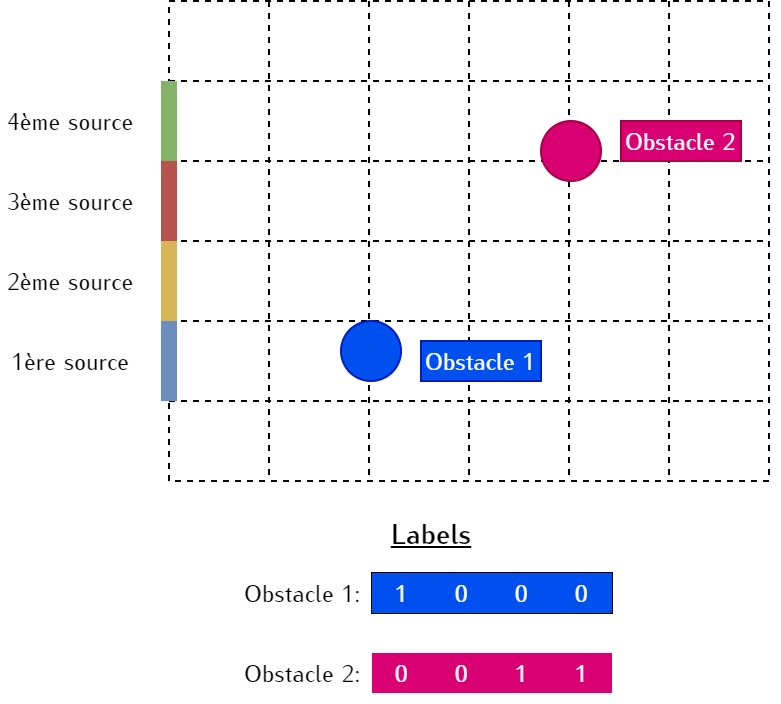
\includegraphics[width=5cm]{Classification}       
            \caption{Labels pour la classification}
            \end{figure}
         \end{column}
         \pause
         \begin{column}{0.35\textwidth}
            \begin{table}[h!]
                \caption{Les scores obtenus}
                \centering
                \begin{tabular}{l l}
                \toprule
                \textbf{Nom} & \textbf{Valeur} \\
                \midrule
                Bin. Acc. & 98.86 \%\\
                Pers. Sév. & 95.45 \%\\
                \bottomrule\\
                \end{tabular}
            \end{table}
         \end{column}
    \end{columns}
\end{frame}

\setbeamercovered{transparent}


%-------------------------------------------------------------------------------
%							SECOND SECTION
%-------------------------------------------------------------------------------

\section{Le transfert radiatif}


\begin{frame}
  \frametitle{Le phénomène du transfert radiatif}

  \scriptsize
Lorsque les photons se trouvent en présence de la matière, trois phénomènes majeurs (caractérisés par leurs opacités) se produisent :

\begin{columns}
  \begin{column}{0.55\textwidth}
    \scriptsize
   \begin{itemize}[<+>]
     \item \textbf{Émission} ($\sigma_e$) : des photons sont émis en réponse aux électrons excités descendants à des niveaux d’énergie plus bas. Plus la température matière est élevée, plus l'émission est importante % Typiquement on ne vas pas retrouver sigma_e dans nos equations car on va se placer dans l'ETL, et on Planck.
     \item \textbf{Absorption} ($\sigma_a$) : à l’inverse, certains photons sont absorbés, les électrons deviennent plus excités (ou se libèrent complètement de leurs atomes), et la matière se réchauffe. À l'équilibre thermique, $\sigma_a = \sigma_e$ % On va considerer en plus l'equilibre chimique ce qui donne l'ETL
     \item \textbf{Dispersion} ($\sigma_c$) : certains photons sont déviés de
     leur trajectoire originale par la matière. Il faut aussi tenir compte de la fonction de distribution angulaire de "scattering" $p(\bm{\Omega^\prime \rightarrow \bm{\Omega}})$ \parencite{Reference3}.
   \end{itemize}
  \end{column}
  % \pause
  \begin{column}{0.45\textwidth}
     \begin{figure}       
      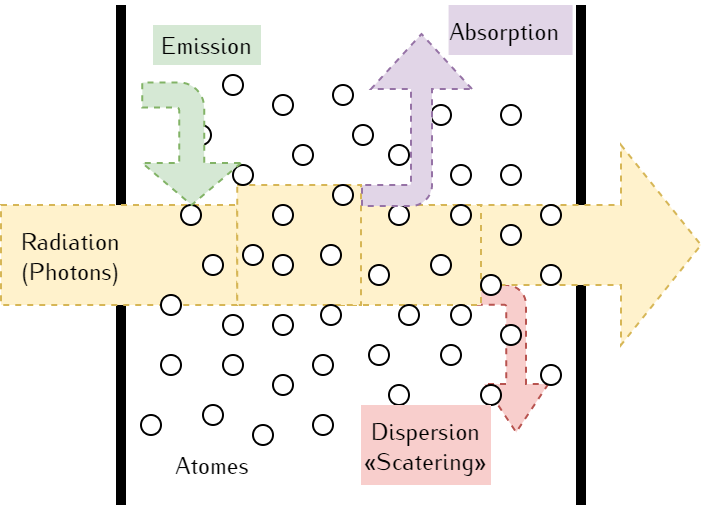
\includegraphics[width=5cm]{TransferRadiatif}       
      \caption{Interaction entre matière et radiation}
    \end{figure}
  \end{column}
 \end{columns}
 
\end{frame}

\begin{frame}
  \frametitle{L'ETR}
  L'équation du transfert radiatif (ETR) est un bilan d'énergie lié au rayonnement au niveau mésoscopique (dans la direction $\bm{\Omega}$). 

  \begingroup
  \scriptsize
  \begin{gather*}
      \begin{aligned}
        \alert<1>{\frac{1}{c} \frac{\partial}{\partial t}I(t,\bvec{x},\bm{\Omega},\nu)} &\alert<1>{+\bm{\Omega}\cdot\nabla_{\bvec{x}} I(t,\bvec{x},\bm{\Omega},\nu)} \\
      &\alert<2>{= \sigma_a(\rho,\bm{\Omega},\nu)\left(B(\nu,T)-I(t,\bvec{x},\bm{\Omega},\nu)\right)} \\
      &\alert<3>{+ \frac{1}{4\pi} \int_{0}^{\infty} \int_{S^2}\sigma_c(\rho,\bm{\Omega},\nu)p(\bm{\Omega}^\prime\rightarrow\bm{\Omega})\left(I(t,\bvec{x},\bm{\Omega}^\prime,\nu)-I(t,\bvec{x},\bm{\Omega},\nu)\right) \, d\bm{\Omega}^\prime \, d\nu}
      \end{aligned}
  % \label{eqn:ETR}
  \end{gather*}
  \endgroup
où :
\begin{itemize}
  \item $I(t,\bvec{x},\bm{\Omega},\nu)$ désigne l'intensité radiative spécifique
  \item $B(\nu,T)$ la fonction de Planck, caractérise l'émission à l'ETL
  \item $\oint p(\bm{\Omega}^\prime\rightarrow\bm{\Omega})\, d\bm{\Omega}^\prime=1$
\end{itemize}

\end{frame}

\begin{frame}
  \frametitle{Le modèle P1}
%   \footnotesize
  Le modèle P1 donne une simplification de l'ETR en vue des simulations. %Le terme 1/3
  \begingroup
  \footnotesize
  \begin{equation*}
      \begin{cases}
        \alert<1->{\partial_tE + c \operatorname {div} \bvec F = c\sigma_a\left(aT^4-E\right)}\\
        \alert<1->{\partial_t\bvec{F} + c \nabla E = -c\sigma_c \bvec{F}} \\
        \alert<1->{\rho C_v \partial_t T = c \sigma_a \left(E-aT^4\right)}
      \end{cases}
  % \label{eqn:P1}
  \end{equation*}
  \endgroup
  où :   % Moins precis que Monte-Carlo ou ordonne discretes; Mais plus rapide et suddisant; sigma
\begin{itemize}
  \item Energie des photons : $E(t,\bvec{x}) = \frac{4\pi}{c} \int_{0}^{\infty} \int_{S^2} I(t,\bvec{x},\bm{\Omega},\nu) \, d\bm{\Omega} \, d\nu$
  \item Flux des photons :    $\bvec{F}(t,\bvec{x}) = \frac{4\pi}{c} \int_{0}^{\infty} \int_{S^2} \bm{\Omega}I(t,\bvec{x},\bm{\Omega},\nu) \, d\bm{\Omega} \, d\nu$  
  % \label{eqn:EFT}
\end{itemize}
\pause
% \normalsize
Ce modèle est :
\begin{itemize}[<+>]
  \item Linéaire et hyperbolique
  \item Macroscopique aux moments (d’ordre 2), dit "gris"
  \item Moins précis qu'un modèle résolut par la méthode de Monte-Carlo 
  \item Peu coûteux et rapide à implémenter
\end{itemize}

\end{frame}

\setbeamercovered{invisible}

\begin{frame}
  \frametitle{Le schéma de "splitting"}
  Le principe :
  \footnotesize
  \begin{enumerate}
    \item<1-> On sépare le problème en temps en deux
    \item<2-> On résout l'étape 1 (réglage de la température) : sur une maille, schéma d'Euler implicite et méthode du point fixe
    $$     \begin{cases}
      \partial_tE + \alert{\underbrace{c \operatorname {div} \bvec F}_{=\,0}} = c\sigma_a\left(aT^4-E\right)\\
      \rho C_v \partial_t T = c \sigma_a \left(E-aT^4\right) 
     \end{cases} $$
    \item<3-> On résout l'étape 2 (partie hyperbolique) : volume finis 2D
    $$     \begin{cases}
      \only<3->{\partial_tE + c \operatorname {div} \bvec F = \alert{\underbrace{c\sigma_a\left(aT^4-E\right)}_{=\,0}}}\\
      \only<3->{\partial_t\bvec{F} + c \ \nabla E = -c\sigma_c \bvec{F}} \\
     \end{cases} $$
    \item<4> \alert {Tout ceci se fait sur le meme pas de temps!}
  \end{enumerate}

\end{frame}
\setbeamercovered{transparent}


\begin{frame}
  \frametitle{Le schéma de "splitting" : Étape 1}
  % Reglage de la temperature 
  \begin{columns}
    \begin{column}{0.5\textwidth}
     À l'itération $n$, on pose $\Theta = aT^4$

      \begingroup
      \normalsize
      \begin{equation*} 
        \begin{dcases}
         \alert<1->{E_j^{q+1} = \dfrac{\alpha E_j^n + \beta \gamma \Theta_j^n}{1 - \beta \delta}} \\
         \alert<1->{\Theta_j^{q+1} = \dfrac{\gamma \Theta_j^n + \alpha \delta E_j^n}{1 - \beta \delta}}
        \end{dcases}
    \label{eqn:Step1}
    \end{equation*}
      \endgroup
      Où
      \tiny
      $\mu_q = \dfrac{1}{T^{3,n} + T^{n}T^{2,q} + T^{q}T^{2,n} + T^{3,q}}$
      \normalsize
    \end{column}
    % \pause
    \begin{column}{0.5\textwidth}
       \begin{center}
        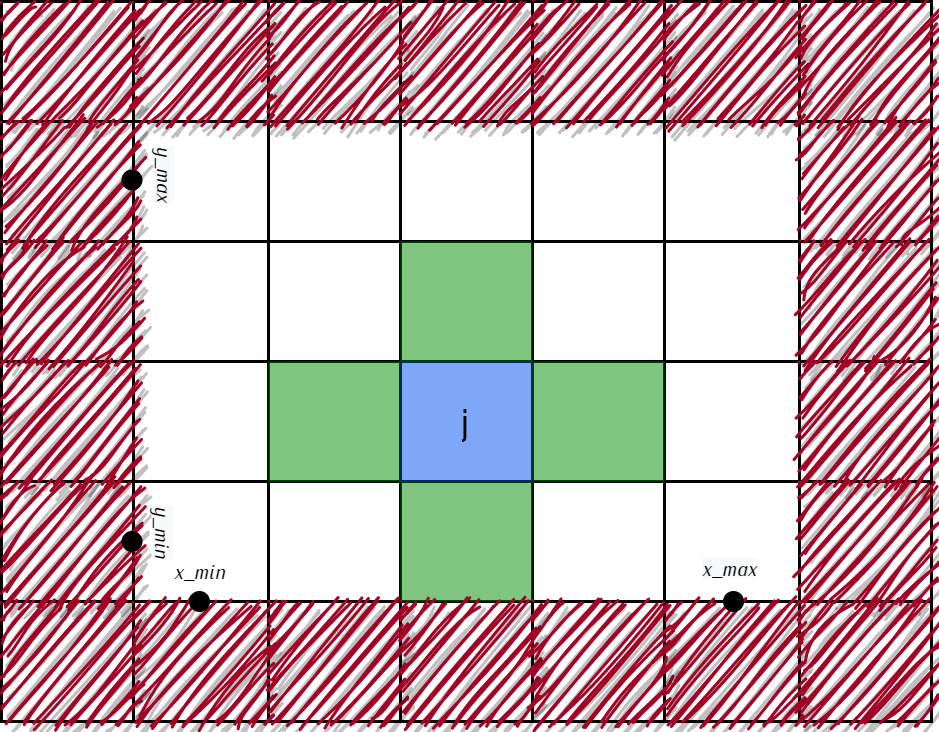
\includegraphics[width=4.5cm]{Dicretisation2D}       
       \end{center}
    \end{column}
   \end{columns}
   \tiny
  $\quad  \alpha = \dfrac{1}{\Delta t \left( \frac{1}{\Delta t} + c \sigma_a \right)} ,\quad 
   \beta = \dfrac{c \sigma_a}{\frac{1}{\Delta t} + c \sigma_a} ,\quad 
   \gamma = \dfrac{\rho_j C_v \mu_q}{\Delta t \left( \frac{\rho_j C_v \mu_q}{\Delta t} + c \sigma_a \right)} \quad , \quad  
   \delta = \dfrac{c \sigma_a}{\frac{\rho_j C_v \mu_q}{\Delta t} + c \sigma_a}.$

   \normalsize
   \begin{columns}
    \begin{column}{1.0\textwidth} 
      \\
      Itération sur $q$ ; convergence vers $E_j^*$ et $\Theta_j^*$ ; $\bvec F_j = \bvec F_j^*$ constant.
    \end{column}
    \begin{column}{0.0\textwidth} 
    \end{column}
  \end{columns}
   
\end{frame}


\begin{frame}
  \frametitle{Le schéma de "splitting" : Étape 2}   % Adaptable aussi en 2D
  \begin{columns}
    \begin{column}{0.6\textwidth}
      \begingroup
      \normalsize
      \begin{equation*} 
          \begin{dcases}
          \alert<1->{E_j^{n+1} = E_j^* + \alpha \sum_k \left( \bvec F_{jk}, \bvec n_{jk} \right)} \\
          \alert<1->{\bvec{F}_j^{n+1} = \beta \bvec F_j^* + \bm{\gamma} E_j^n + \delta \sum_k E_{jk} \bvec n_{jk}}
          \end{dcases}   
      % \label{eqn:Step2}
      \end{equation*}
      Avec :
      \newline
      % \begingroup
      \scriptsize
    
      % \begin{gather*}    
      % \begin{aligned} 
        $\alpha = -\frac{c \Delta t}{\left| \Omega_j \right|}, \linebreak
        \beta = \frac{1}{\Delta t} \left( \frac{1}{\Delta t} + c \sum_k M_{jk} \sigma_{jk} \right)^{-1}, \linebreak
        \bm{\gamma} = \frac{c}{\left| \Omega_j \right|} \left( \frac{1}{\Delta t} + c \sum_k M_{jk} \sigma_{jk} \right)^{-1} \left( \sum_k l_{jk} M_{jk} \bvec n_{jk} \right) \linebreak
        \delta = -\frac{c}{\left| \Omega_j \right|} \left( \frac{1}{\Delta t} + c \sum_k M_{jk} \sigma_{jk} \right)^{-1}$
    %   \end{aligned}
    % \end{gather*}

    \endgroup
      
    \end{column}
    % \pause
    \begin{column}{0.4\textwidth}
      % \begin{figure}
      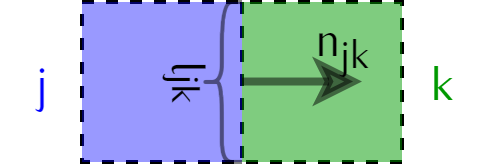
\includegraphics[width=5cm]{Interaction2D}       
        % \caption{Interaction entre deux mailles}
      % \end{figure}
       \begin{center}
        \begingroup
        \tiny
        \begin{align*}
          \left(\bvec F_{jk}, \bvec n_{jk} \right) &= l_{jk} M_{jk} \left( \frac{\bvec F_j^n \cdot \bvec n_{jk} + \bvec F_k^n \cdot \bvec n_{jk}}{2} - \frac{E_k^n - E_j^n}{2} \right) \\
          E_{jk} \bvec n_{jk} &= l_{jk} M_{jk} \left( \frac{E_j^n + E_k^n}{2} - \frac{\bvec F_k^n \cdot \bvec n_{jk} - \bvec F_j^n \cdot \bvec n_{jk}}{2} \right) \bvec n_{jk} \\
        %  \end{align*}
        %  \begin{align*}
          M_{jk} &= \frac{2}{2 + \Delta x \sigma_{jk}}  \\
          \sigma_{jk} &= \frac{1}{2} \left( \sigma_c(\rho_j,T_j^n) + \sigma_c(\rho_k,T_k^n) \right)
         \end{align*}
        \endgroup
       \end{center}
    \end{column}
   \end{columns}
\end{frame}

\begin{frame}
  \frametitle{Implémentation C++}
  \begin{columns}
    \begin{column}{0.5\textwidth}
      \scriptsize
      \begin{itemize}
        \item Temps final = 0.01 \si{sh} %\textit{(1 shake (\si{sh}) = $10^{-8}$ secondes)}
        \item $c = 299$ [\si{\cm \per sh}]
        \item $a = 0.01372$ [\si{g \per cm \per sh^2  \per keV }]
        \item $C_v = 0.14361$ [\si{Jerk \per\g \per keV}] % \textit{(1 \si{Jerk} = 1\si{m \per \s\cubed})}
        \item La densité $\rho$ est un signal complet [\si{\g\per\cm\cubed}]
        \item $\sigma_a = \rho T$ [\si{\per\cm}]
        \item $\sigma_c = \rho T$ [\si{\per\cm}]
        \item $T_0, T_{gauche} = 5$ [\si{keV}] % \textit{(en termes de température, 1 \si{keV} = 11605 \si{K})}
        \item $E_0 = aT_0^4$ [\si{g \per \cm \per sh^2}]
        \item $E_{gauche^*} = aT_{0}^4 + 5 \sin (2 k \pi t)$ [\si{g \per \cm \per sh^2}]
        \item $\bvec{F}_0, \bvec{F}_{gauche} = \bvec{0}$ [\si{g \per sh^2}]
        \item Sorties libres sur les autres bords
      \end{itemize}
    \end{column}


    \begin{column}{0.5\textwidth}
       \begin{figure}
        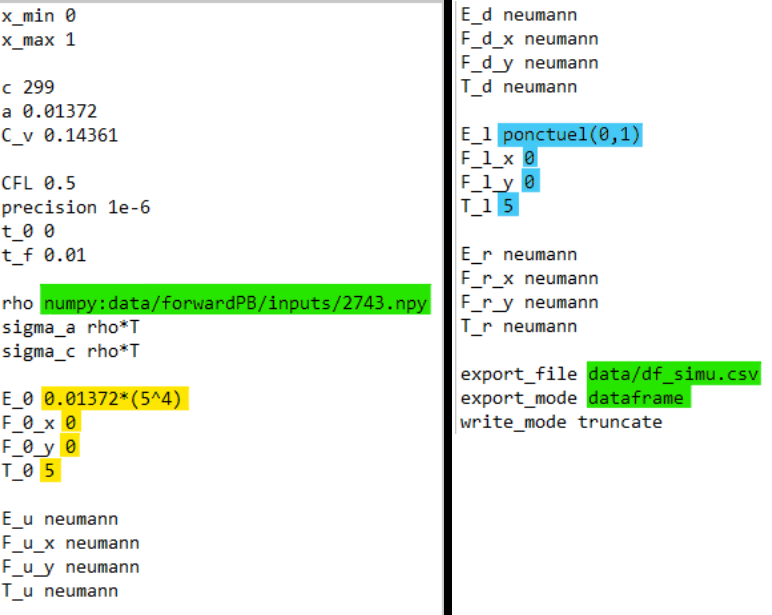
\includegraphics[width=5cm]{SimuCFG}   % EN 2D    
        \only{\caption{Exemple de fichier configuration}}
      \end{figure}
    \end{column}
   \end{columns}

\end{frame}



%-------------------------------------------------------------------------------
%							THIRD SECTION
%-------------------------------------------------------------------------------

\section{Le Vnet}


\begin{frame}
    \begin{figure}
        \includegraphics<1->[width=11cm]{Vnet.png}         
      \end{figure}
\end{frame}


% 
%-------------------------------------------------------------------------------
%							FOURTH SECTION
%-------------------------------------------------------------------------------


% 
%-------------------------------------------------------------------------------
%							FITH SECTION
%-------------------------------------------------------------------------------


% %-------------------------------------------------------------------------------
% %							THANK YOU NOTE
% %-------------------------------------------------------------------------------

\begin{frame}
  \Large
  \centering
  Merci pour votre attention durant cette mini-partie. La suite dans le notebook...

\end{frame}

% %-------------------------------------------------------------------------------
% %							THE BIBLIOGRAPHY
% %-------------------------------------------------------------------------------
% \appendix   % Pour retirer les references de la bare de navigation
% \vspace*{0.5mm}
% \printbibliography


\end{document}
